\documentclass{article}
\usepackage[top=1.00in, bottom=1.0in, left=1.00in, right=1.00in]{geometry}
\renewcommand{\baselinestretch}{1.1}
\usepackage{graphicx}
\usepackage{float}
\usepackage{natbib}
\usepackage{amsmath}
\bibliographystyle{..//refs/styles/besjournals.bst}
\parindent=24pt
\def\labelitemi{--}
\usepackage{lineno}
\linenumbers
\usepackage{xr-hyper}
\externaldocument{FLSshort_supp}

\title{Reconciling competing hypotheses regarding flower-leaf sequences in temperate forests for fundamental and global change biology}

\author{D.M. Buonaiuto, I. Moralles Castilla, E.M. Wolkovich}

%3472 words
\begin{document}
\maketitle
\section*{Abstract}
Phenology is a major component of an organism's fitness. While individual phenological events affect fitness, growing evidence suggests that the relationship between events may be equally or more important. This may explain why deciduous woody plants exhibit considerable variation in the order of reproductive and vegetative events, or flower-leaf sequences (FLSs). Research suggests that FLSs are adaptive, with several competing hypotheses to explain their function. Reconciling these hypotheses has been impeded by how FLS patterns are described and defined. Here, we advance the existing hypotheses to account for the FLS variation in nature and evaluate them with case studies. Our inquiry provides three major insights towards a new framework for understanding FLSs. First, we find concurrent support for multiple hypotheses, suggesting progress can come from studies addressing overlapping hypotheses. Second, support for FLS hypotheses is sensitive to how FLSs are defined, with quantitative definitions proving most useful. Finally, we identify the limits of trait-based hypothesis testing. We highlight how adopting an intra-specific approach and evaluating fitness consequences of FLS variation could quickly determine the major drivers, with cascading benefits to improving predictions of how climate change will alter FLSs and thereby re-shape plant communities and ecosystems.

\section*{Introduction}
Phenology, the timing of seasonal life cycle events, allows organisms to synchronize life-history transitions with optimum environmental conditions \citep{Forrest2010}, and is a critical component of ecosystem structure and function \citep{Cleland2007,Piao2007}. Recent work in woody plant phenology has shown that it is not only individual phenological stages that affect these processes, but also the relationships between them \citep{Ettinger2018}.\\

\noindent One phenological relationship that has long received scientific interest \citep[see][]{Robertson1895} and, recently, increased attention in the literature \citep{Savage2019, Gougherty2018} is the flower-leaf phenological sequence (FLS) of deciduous woody plants. In a typical model of plant life-history, vegetative growth precedes reproduction. However, for many species in the forests of Eastern North America, it is not the green tips of new shoots that mark the commencement of the growing season, but the subtle reds and yellows of their flowers. This flowering-first FLS is common in these forests, and its prevalence suggests that this FLS has adaptive significance \citep{Rathcke_1985}.\\ 

\noindent Understanding this phenological pattern is necessary and timely because anthropogenic climate change is altering FLSs (Fig. \ref{fig:climchange}). Long-term observations show the number of days between flowering and leafout is increasing as a result of climate change, but the rate of change differs up to five-fold among species (Fig. \ref{fig:climchange}).  If FLSs are indeed an important component of woody plant fitness, this inter-specific variation will exacerbate fitness differences between species, influencing which species will persist under altered climate conditions.\\

\noindent Long-term data also highlight high within species variability in FLSs. Despite recent advances in understanding the physiology and evolution of FLS \citep{Gougherty2018,Savage2019}, most research has ignored this variability---potentially stymieing efforts to predict how FLS patterns will respond to climate change. While some authors present general correlations between flowering and leafing phenology \citep{Lechowicz_1995, Ettinger2018}, fine-scale FLS variability has never been evaluated. We suggest that characterizing intra-specific variation in FLS will not only improve our ability to predict how FLS patterns will change in the future, but also allow for a more biologically relevant evaluation of the current FLS hypotheses, revealing avenues for future, direct hypothesis testing.\\

\noindent Here we 1) review the hypotheses of woody plant FLSs and their respective predictions, 2) compare the biological basis of the current FLS framework to our proposed framework based on intra-specific, quantitative measures of FLS, 3) test our framework with a detailed case study of long-term phenology records from Harvard Forest in Petersham, MA, and 4) make recommendations to improve future study of FLSs.
\section*{FLS hypotheses and their predictions}
\section*{Hypotheses of FLS}
\subsubsection*{ Wind pollination}
\noindent The most prevalent FLS hypothesis suggests that flowering-first is an adaptation for wind-pollination, with leafless flowering allowing for more efficient pollen transfer \citep{Whitehead1969, Spurr1980,Friedman2009}. The primary evidence for this hypothesis comes from pollen diffusion studies \citep[e.g., particle movement through closed and open canopies,][]{Niklas1985,Nathan2005, Milleron2012} and suggests canopy structure does indeed encumber pollen movement. This hypothesis predicts a strong association between FLS and pollination syndrome.
\subsubsection*{Water dynamics}
\noindent Another hypothesis suggests that flowering before leaf development is an adaptation to reduce water stress caused by concurrently maintaining floral hydration and leaf transpiration. \citep{Franklin2016}. Observations of flowering in the dry tropics where this FLS pattern is also common confirm that the timing of flowering in these taxa is associated with a water status recovery due to leaf drop \citep{Borchert1983,Reich1984}, but that this relationship is not physiologically mechanistic \citep{Franklin2016}. This hypothesis predicts a strong relationship between FLS and metrics of drought tolerance.

\subsubsection*{Early flowering}
\noindent A third possibility is that the flowering-first FLS is a physiological byproduct of selection for early flowering \citep{Primack1987}. Here, there is no advantage to a species flowering before or after leafing, as long as the absolute flowering time is the same. \citet{Primack1987} notes that flowering-first species tend to also have large seed mass and lack primary seed dormancy for germination, traits associated with early flowering in general. This raises the possibility that this FLS may simply be one component of a larger suite of early flowering traits. Recent work from \citet{Savage2019} demonstrated that spring flower phenology is less constrained by prior phenological events than leaf phenology, which would allow selection to drive flowering into the early season, producing the the flowering-first FLS. Given this hypothesis, we would expect a strong relationship between a flowering-first FLS and early flowering in general.
\subsubsection*{Phylogenetics} 
\noindent Finally, it is also possible that FLSs are highly conserved traits and the preponderance of flowering-first in the temperate zone is a product of phylogenetic representation of the region rather than an adaptive aspect of the trait. In a recent analysis, \citet{Gougherty2018} found strong phylogenetic clustering in FLS variation. Given this hypothesis, we would expect to see only weak relationships between FLS and the above mentioned traits and a strong phylogenetic signal.\\

\noindent Despite decades of inquiry, only limited progress has been made towards any consensus for these hypotheses. Many studies only test a single hypothesis, making comparison between them difficult. In contrast, studies testing multiple hypotheses have generally found support for multiple hypotheses \citep[see][]{Bolmgren2003,Gougherty2018}. We argue that this lack of resolution stems from the fact that the current way that FLS patterns are conceptualized is not compatible with the biological processes underlying the very FLS variation that research aims to test.

\section*{The current FLS framework and its limitations}
Under the current framework, FLSs are described qualitatively, and defined at the species level. This inherently introduces observer and interpreter bias into FLS data, and fails to capture underlying biology that structures FLS. Below, we highlight three main spurious assumptions of the current FLS framework and suggest alternatives for describing FLS patterns.
\subsection*{Assumption I: FLS patterns are simple to describe and biologically meaningful:}
In the current framework, there are three main FLS categories: flowers before leaves (hysteranthy, proteranthy, precocious flowering); flowers with leaves (synanthy); and flowers after leaves (seranthy) \citep{Lamont2011, Heinig1899}. Some data sources \citep[e.g.][]{Burns1990,Barnes2004} include additional categories: ``flowers before/with leaves" and ``flowers with/after leaves", but it is unclear whether these categories describe intermediate FLS patterns or FLS variability in these species. While these categories are conceptually reasonable, applying them to real phenological sequences is not always so straightforward.\\

\noindent Both reproductive and vegetative phenological sequences consist of multiple sub-stages, and this introduces significant ambiguity into how we interpret qualitative FLS descriptions. Consider a species with the following FLS:\\

\begin{center}
\textbf{flower budburst}$\rightarrow$ \textbf{leaf budburst}$\rightarrow$ \textbf{first flowers open} $\rightarrow$ \textbf{leafout} $\rightarrow$ \textbf{peak flowering} $\rightarrow$ \textbf{end of leaf expansion} \\
\end{center}

\noindent Observers could justifiably classify this species as: 1) Hysteranthous because flower budburst proceeds leaf budburst, 2) Synanthous because flowers open during the budburst-leafout inter-phase 3) Seranthous because peak flowering occurs after leafout. This problem extends beyond this simple example to real datasets, \citep[e.g.][]{OKeefe2015} where the same ambiguities exist (Fig \ref{fig:HFmeans}). Not surprisingly then, different sources may classify the same species differently. We compared species-level FLS descriptions in two of the most comprehensive records of FLS, \underline{Michigan Trees} and its companion volume \underline{Michigan Shrubs and Vines} (MTSV) \citep{Barnes2004,Barnes2016} with \underline{The USFS Silvics Manual Volume II} \citep{Burns1990}. Of the 49 overlapping species, 30\% were classified differently. Such different classifications could reflect interesting temporal or geographic variability in FLSs, but---given current definitions---they could equally be an artifact of observer decision-making.\\

\noindent Categorization can often introduce biases in analyses \citep{Naggara2011,Royston2006}, and in this case, the FLS hypotheses themselves may suggest different boundaries than the ones prescribe by the traditional framework. Given that the most complete FLS datasets come from regional guide books and floras, FLS categories were likely determined to aid with plant identification rather than to detail biological processes. For example, the wind-pollination hypothesis hinges on the fact that leaves create a substantial physical disruption to pollen transfer, a premise that would not necessarily be true for the early stages of leaf expansion when tiny leaf primordia would have little impact on environmental structure. Rather, trees that flower during the early stages of leaf expansion should gain similar advantage to those who complete their flowering before any leaf activity. Alternatively, because transpiration intensifies as soon as leaves begin to expand \citep{Breda1996,Wang2018}, there should a cost to maintaining floral structures during any stage of leaf activity, and only species whose flowering occurs before any leaf expansion would gain a drought advantage. Given the biological processes underlying these hypotheses, statistical relationships between FLS and traits will fluctuate depending on where category boundaries are defined. Important associations may be missed entirely if, as in the case of the current categories, the imposed boundary does not match the biological processes.

\subsection*{Assumption II: There are no meaningful differences within FLS categories}
 Consider the selection of species from Harvard Forest depicted in figure (Fig. \ref{fig:vizzy}). According to the current framework, these species are classified simply based on sequence, but this ignores any other measure of time (Fig. \ref{fig:vizzy}a). Biology, however, has continually shown that the length of time also matters \citep{Inouye2019}, and when the timing between reproductive and vegetative events are quantified (Fig. \ref{fig:vizzy}b), it is clear that the FLSs of these species within each category are are highly contrasting. This substantial inter-specific variation, previously obscured by categorization, could in reality be the fingerprint of selection on FLSs. %This inter-specific variation can, and should be leveraged for FLS hypothesis testing as will be discussed below.

\subsection*{Assumption III: FLS variation is a species level trait}
In the current framework, FLS categories are assigned at the species level. We investigated individual FLS variation at Harvard Forest \citep{OKeefe2015}, and found that the time between flowering and leaf activity varied by as much as several weeks between individuals and years, and in some species the sequence itself regularly switched across time and individuals  (Fig. \ref{fig:vizzy} c). A key component of understanding FLS is determining what drives this level of variability and how it affects the biological functions of individuals. It is clear that considering FLS variability at only higher taxonomic levels obscures important realities about the biology of this phenological trait that may be instrumental for better tests of the FLS hypotheses.\\

\noindent Under the current framework, any statistical relationship between FLS and other traits is biased by the subjectivity of the original observer, the modeler, and the possibility that the associations being tested do not reflect the biological processes that shape FLS. We compared traits associated with hysteranthy in the USFS and MTSV datasets. We applied two alternative FLS categorizations; physiological hysteranthy, which allowed for no overlap between floral and leaf phenophases, and functional hysteranthy, which allowed for a degree of overlap. We found the strength of associations between FLS and predictors is highly sensitive to how FLSs were defined (Fig: \ref{fig:muplots.USMT}, e.g. pollination syndrome). With the current framework, any similar analyses would be subject to these biases, and inferences from them may be tenuous. \\

\section*{A new framework for FLS}
The shortcomings of the current FLS framework can be rectified with a shift from categorical, species-level descriptions of FLS to continuous individual-level quantification. The primary reason for this shift is logical: if researchers seek to understand the biological processes driving FLS patterns, we will be the most successful if we use the most biologically relevant measures. Making this change should improve and clarify inferences from traits association models like the ones presented above. Additionally, a quantitative, intra-specific framework offers secondary advantages and novel avenues for fine-tuning FLS hypotheses.\\

\noindent In addition to addressing substantial inter-specific differences in FLS, quantitative measures of phenology \citep[e.g. the BBCH scale,][]{Finn2007} standardize data across time and space, observer, and analyst. Adopting such measurements in the study of phenological sequences would allow for FLS patterns to be compared across larger temporal, geographic, and taxonomic scales, giving researchers more power to accurately address questions about FLS variation.\\

\noindent Addressing intra-specific variation in FLSs augments the existing FLS hypotheses and generates new, testable predictions. A core concept of the theory of natural selection is that the same selective forces that ultimately generate inter-specific differences opperate on individual variation \citep{Dobzhansky1982, Schluter1996}; therefore, drivers of selection should be detectable across the intra- to inter- specific continuum. For example, in the case of FLS, if at the inter-specific level, the water dynamics hypothesis predicts a relationship between drought tolerance and FLS, then at the intra-specific level, inter-annual or population-level variation in FLS should correlate with variation in water availability. Given that phenology studies are often taxonomically and geographically biased \citep{Wolkovich2014,Willis2017} and community analyses of FLS are sensitive to which species are included (Fig. \ref{fig:muplots.USMT}), testing FLS hypotheses within species has potential to generate more reliable results. If instead, results from intra-specific analyses systematically contradict inter-specific studies, this contrast would be a valuable contribution to the growing body of literature attempting to understand the biological implications of scale-dependent drivers of evolution \citep[e.g.,][]{Violle2012,Shipley2016,Anderegg2018}.  \\
 
\noindent Finally, one of the challenges of inter-specific comparisons that can be mitigated by an intra-specific approach is that species evolve a suite of traits for any function, and unmeasured traits might bias results \citep{Davies2019}. For example, wind-pollinated species could compensate for pollen intercepted by a seranthous FLS by over-producing pollen or through self-pollination, and omitting such trade-offs from analyses would bias inter-specific comparisons. Focusing on FLS variation within species holds most other traits relatively equal, which will allow researchers to move beyond simple trait-correlation analyses and begin to assess the consequences of FLS variation. This shift in focus is necessary not only to more accurately validate FLS hypotheses, but also to predict the effects of changing FLS patterns with climate change. \\


\section*{Testing the new framework}

To date, quantitative FLS variability below the species level has not been addressed. To address this gap, we supplement our literature review with several analyses using the phenological records from Harvard Forest \citep{OKeefe2015}. First, to test our proposed framework, we modeled the associations between FLS and hypothesis-relevant traits using both the classic, categorical FLS framework and our new, quantitative one. With the classic approach, we found strongest support for the early flowering hypothesis, good support for the wind pollination hypothesis and poor support for the water dynamics hypothesis, with no substantial interactions between predictors and a strong phylogenetic structure to FLS (Fig. \ref{fig:muplots.HF}) . These results are qualitative similar to models from two other large categorical FLS datasets (Fig. \ref{fig:muplots.USMT}). \\

\noindent The quantitative version of the model paints a more complex picture of the function of FLSs, highlighting key biological insights obscured by categorization. While the main effects and phylogenetic signal are generally in line with those from the categorical model, here we detected a signal for the water dynamics hypothesis. This suggests that. while drought tolerance may not play a major role in determining whether or not flowering happens before leaf expansion, it may contribute to determining the time between these phenophases. Most significantly, in this model we identify strong interactions between predictors. While early flowering is associated with hysteranthy in all species, this effect is even more pronounced in wind-pollinated taxa. (Fig. \ref{fig:muplots.HF}) Marginal effects from this model demonstrate that water dynamics drive FLS patterns of biotically-pollinated taxa but not wind-pollinated taxa (Fig. \ref{fig:apcs}). \\

\noindent These systematic differences between pollination syndromes are informative. Many of the biotically-pollinated species of the temperature forests trace their bio-geographic origins to the tropical regions \citep{Daubenmire1972} where the water dynamics hypothesis originated \citep{Janzen1967,Franklin2016}. In particular, many biotically-pollinated, hysteranthous species in the temperate zone are geographic outlyers from largely tropical clades (e.g. \textit(Fabaceae),\textit(Lauraceae),\textit(Annonaceae). It may be that for these taxa, hysteranthy developed in a warmer, drier selection environment and bears no functional similarity to hysteranthous flowering in wind-pollinated species that predominately evolved in the temperate zone. While beyond the scope of this analysis, the bio-geography behind our findings suggests a more complex story of parallel evolution, bio-geographic history, and community assembly in hysteranthous flowering than can be encompassed by any single FLS hypothesis.\\

\noindent Given the the emergence of support for the water dynamics hypothesis under the intra-specific, quantitative FLS framework, we next leveraged the inter-annual FLS variation at Harvard Forest to test one of the modified, intra-specific predictions of the water dynamics hypothesis. As predicted, we found a negative association between FLS variation and annual precipitation at Harvard Forest. However, we estimated it would take a change of approximately 100 centimeters in annual precipitation to drive a day difference in FLS, suggesting annual precipitation is not a major contributor to the observed inter-annual FLS variation.

These result suggest that even if water dynamics shaped FLS in some temperate taxa on the evolutionary time-scale, it does not appear to be a major driver of FLS variation on an ecological one. Given this, it may be that hysteranthy in biotically-pollinated species in the temperate zone is maintained because there is no strong selection against it, or it has come to serve a different function. Hysteranthous flowering may expand the temporal niches available to species, partitioning inter-specific competition for pollinators, or it may be a useful tool for attracting them. For example, there is some evidence that hysteranthous species invest less in floral resources than seranthous sister taxa \citep{Gunatilleke1984}, suggesting that perhaps their flowers are easier for pollinators to locate. While these explanations are still purely speculative, they are readily testable with our new framework.\\

\noindent Our findings suggest that the fact that previous studies tend to find support for multiple hypotheses \citep{Bolmgren2003,Gougherty2018,Savage2019} is not simply a methodological artifact but rather a result consistent with the biological processes that shape FLS. Using available data, we have demonstrated the advantages of a new conceptual framework for the study of FLSs based on quantitative measures of individual variation in FLS patterns. Using these methods, we found that in accordance with previous work, flowering time and pollination syndrome are important drivers of hysteranthy \citep{Gougherty2018}. We also found support for the water dynamics hypothesis in the evolutionary history of biotically-pollinated taxa, and identified several new, testable hypotheses regarding the biological nuances of FLSs. Together, these results provide a more comprehensive picture of where our understanding of this phenological trait is currently, and where it needs to go. Below we highlight three characteristics of FLS that we suggest, utilizing this new framework, should be incorporated into future research to improve our fundamental knowledge about this important life-history trait and better predict how alterations to FLSs will impact species in an era of global change.
\section*{The Future of FLS:}
\subsubsection*{Multiple hypotheses explain FLSs}

\noindent Our results underscore other lines of evidence that show multiple hypotheses should be the starting point for future FLS research. While there is certainly value to broad taxonomic studies, and future large-scale analyses should continue, the consistent support for multiple hypotheses shows there are limits to the utility of these kinds of studies. We suggest that it is better to explore the evolutionary dynamics of hysteranthy with a more mechanistic approach, which may mean utilizing a more taxonomically-restricted focus. The significance of interaction terms in our case study suggests that a promising option is to look within the hypotheses to address sub-grouping of taxa in which overlap between hypotheses could be controlled. For example, we know that wind-pollination efficiency is not driving hysteranthous flowering among biotically-pollinated taxa, so considering this group of species alone may provide a stronger test of competing hypotheses. Incorporating a more explicit phylo-bio-geographic approach would be instructive at this level; there are phylo-geographic commonalities between many of the biotically-pollinated hysteranthous species in the Eastern flora, and we might better understand the function of FLS variation in these species by investigating FLS variation in their sister-taxa in their regions of origin.\\ 

\subsubsection*{FLS and fitness}
Even with focused work on sub-groupings of species, inter-specific trait-association models can only can take us so far. As in most other areas of plant biology examining traits, research is hampered by the difficulty of knowing which are the right traits \citep{Violle2007}. For example, we used minimum precipitation across a species' range, one of the only available quantitative drought metrics at the scale of large inter-specific models, to represent the water dynamics hypothesis, but we have no way of knowing for certain that this is actually a good proxy for drought tolerance. \\

\noindent While trait associations point to past selection, fitness is the driver of trait evolution, and at the core of each FLS hypothesis is a fitness prediction. By utilizing intra-specific comparisons and continuous measurements of FLS, we can move beyond trait associations and test the fitness consequences of FLS variation. As we discussed above, the theory of natural selection dictates that if under selection, variability in hysteranthy should lead to variability in fitness outcomes at the intra-specific level. For example, the wind pollination hypothesis predicts that with all else equal, years with increased time between flowering and leafing should correlate with more pollination success. The water dynamics hypothesis suggests hysteranthous populations with a consistently larger time between flowering and leafing should better tolerate drought. These predictions could be directly assessed through well-designed experiments and field studies, providing a new avenue to test the existing hypotheses and better understand the implications of shifting FLSs.\\

\subsubsection*{FLS and physiology} 
Decades of research shows that both floral and vegetative phenological events are cued by temperature and photoperiod \citep{Forrest2010, Flynn2018}, suggesting they are under shared genetic and physiological control. But to yield the FLS variation seen in nature, there must be systematic differences in reproductive and vegetative phenological responses to the environment. Researchers can use intra-specific variation in FLS to identify which cues dominate each phenological process and better understand the underlying genetic and physiological constraints that structure phenological sequences.\\

\emph{Conclusions:} Our proposed framework provides a path to understanding the drivers of FLSs in woody plants. Through examining FLS variation in more targeted taxonomic assemblages and using quantitative data with mechanistic metrics, we can refine the existing FLS hypotheses and better comprehend the causes and consequences of FLS variation at multiple taxonomic scales. This is an essential step towards a more complete understanding of the fundamental biology of temperate woody plants, and for predicting the fate of these species as global climate continues to change.

\bibliography{..//refs/hyst_outline.bib}
 
\pagebreak

\section*{Figures}
\begin{figure}[h!]
    \centering
 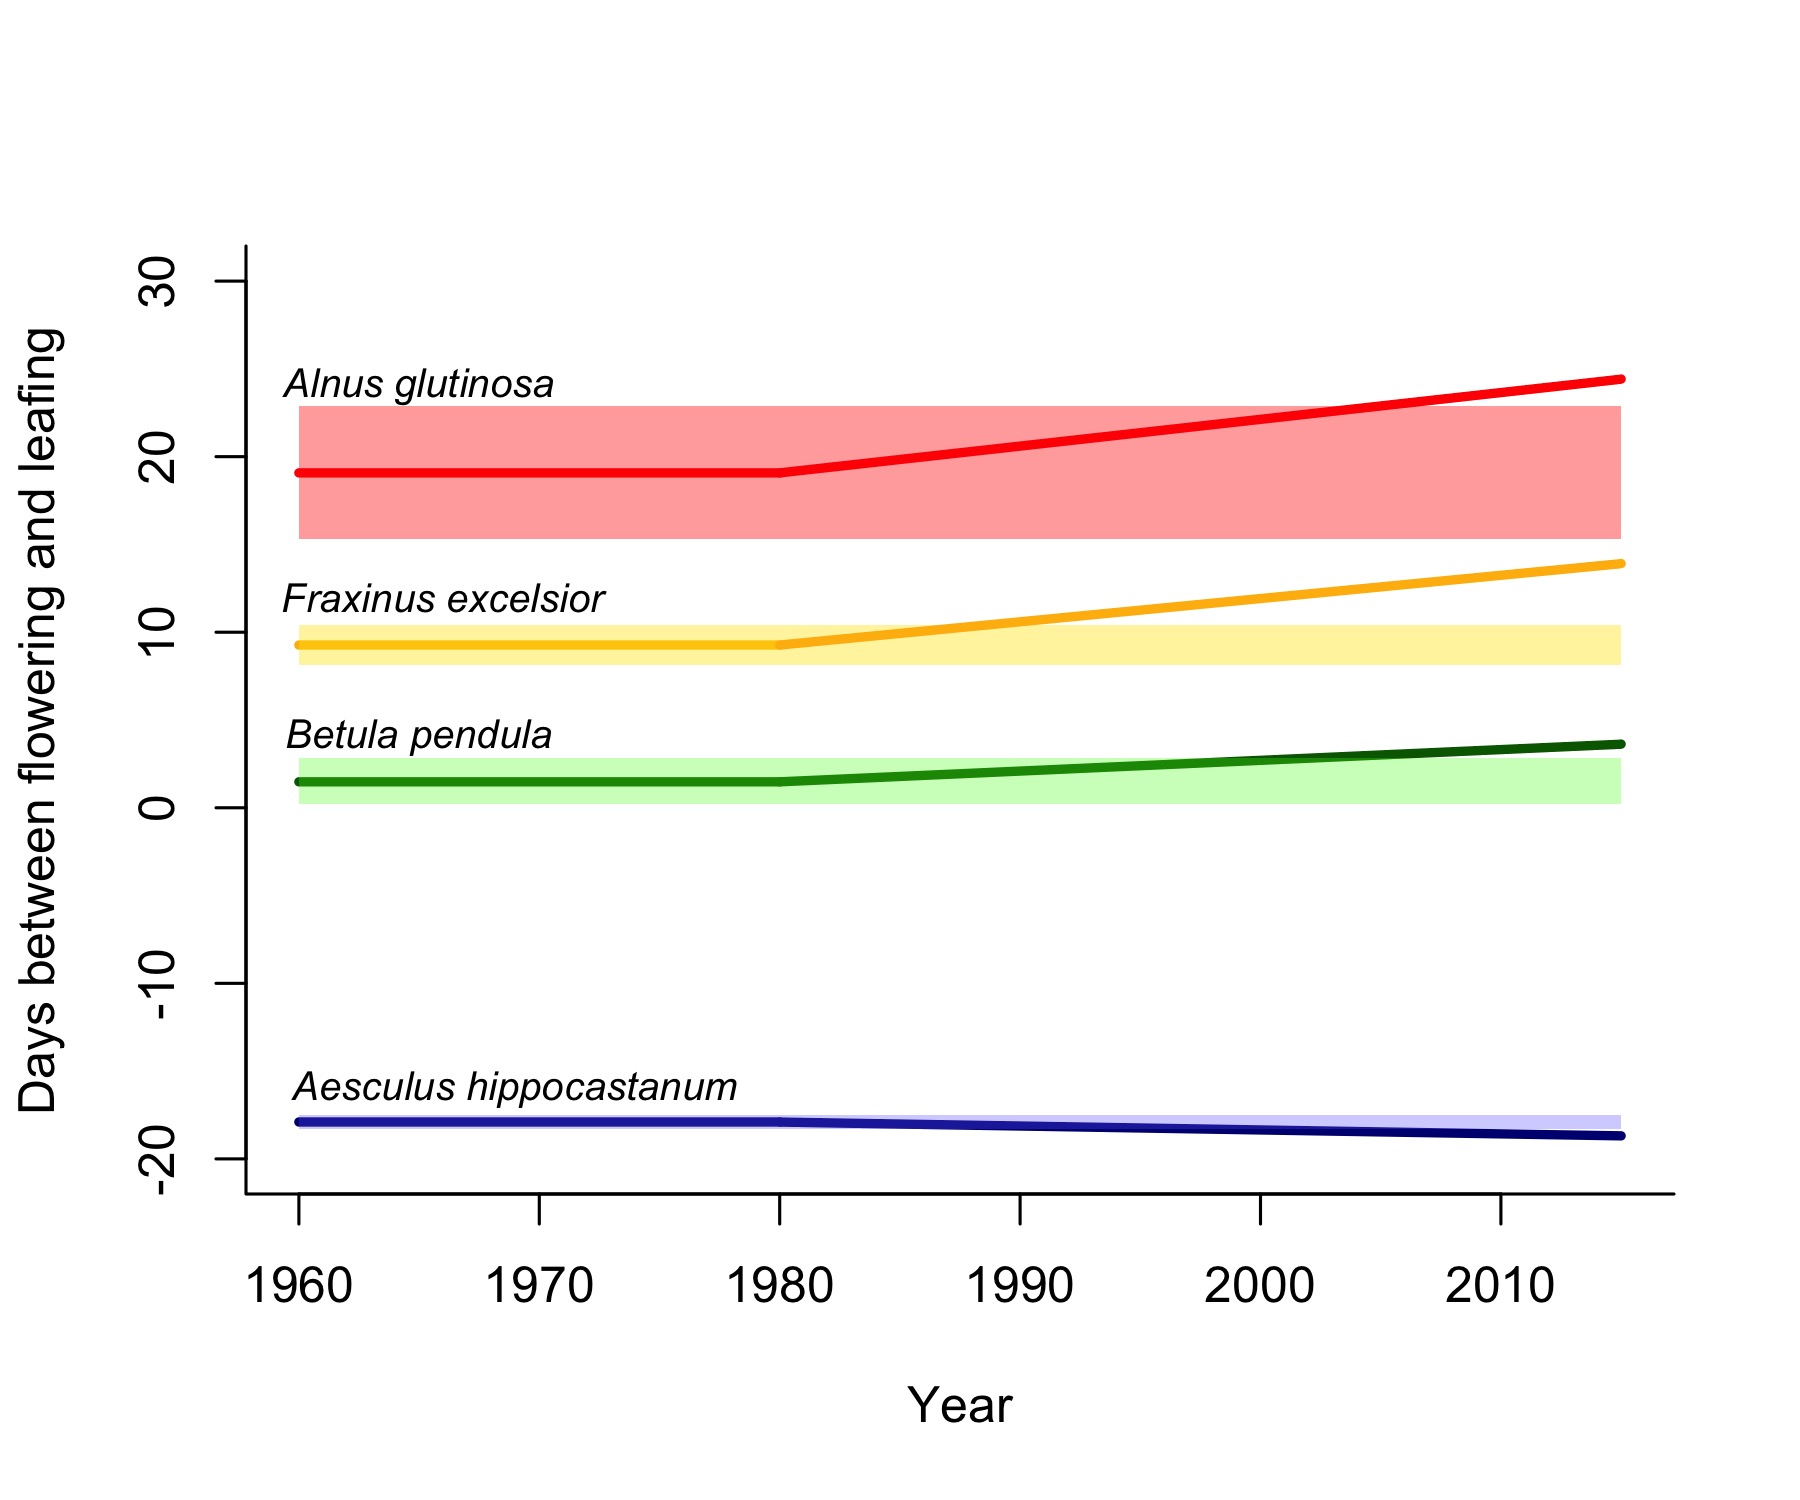
\includegraphics[width=\textwidth]{..//PEP725/FLS_climate_change.jpeg} 
    \caption{\textbf{FLSs across Europe for four tree species from 1960 to 2015 suggests climate change has generally increased the time between flowering and leafing}, but the direction and rate of change differs across species, which may exacerbate fitness differences within forest communities. To detect the effect of climate change on average FLS, we used models that allow for shifts in FLS after 1980. Lines represent the mean trend in FLS per species, and the highlighted regions indicate historic range of FLS variability (95\% credible intervals of the pre-1980 average) from the PEP725 database \citep{PEP725}.}
    \label{fig:climchange}
\end{figure}
 
 \begin{figure}[h!]
        \centering
          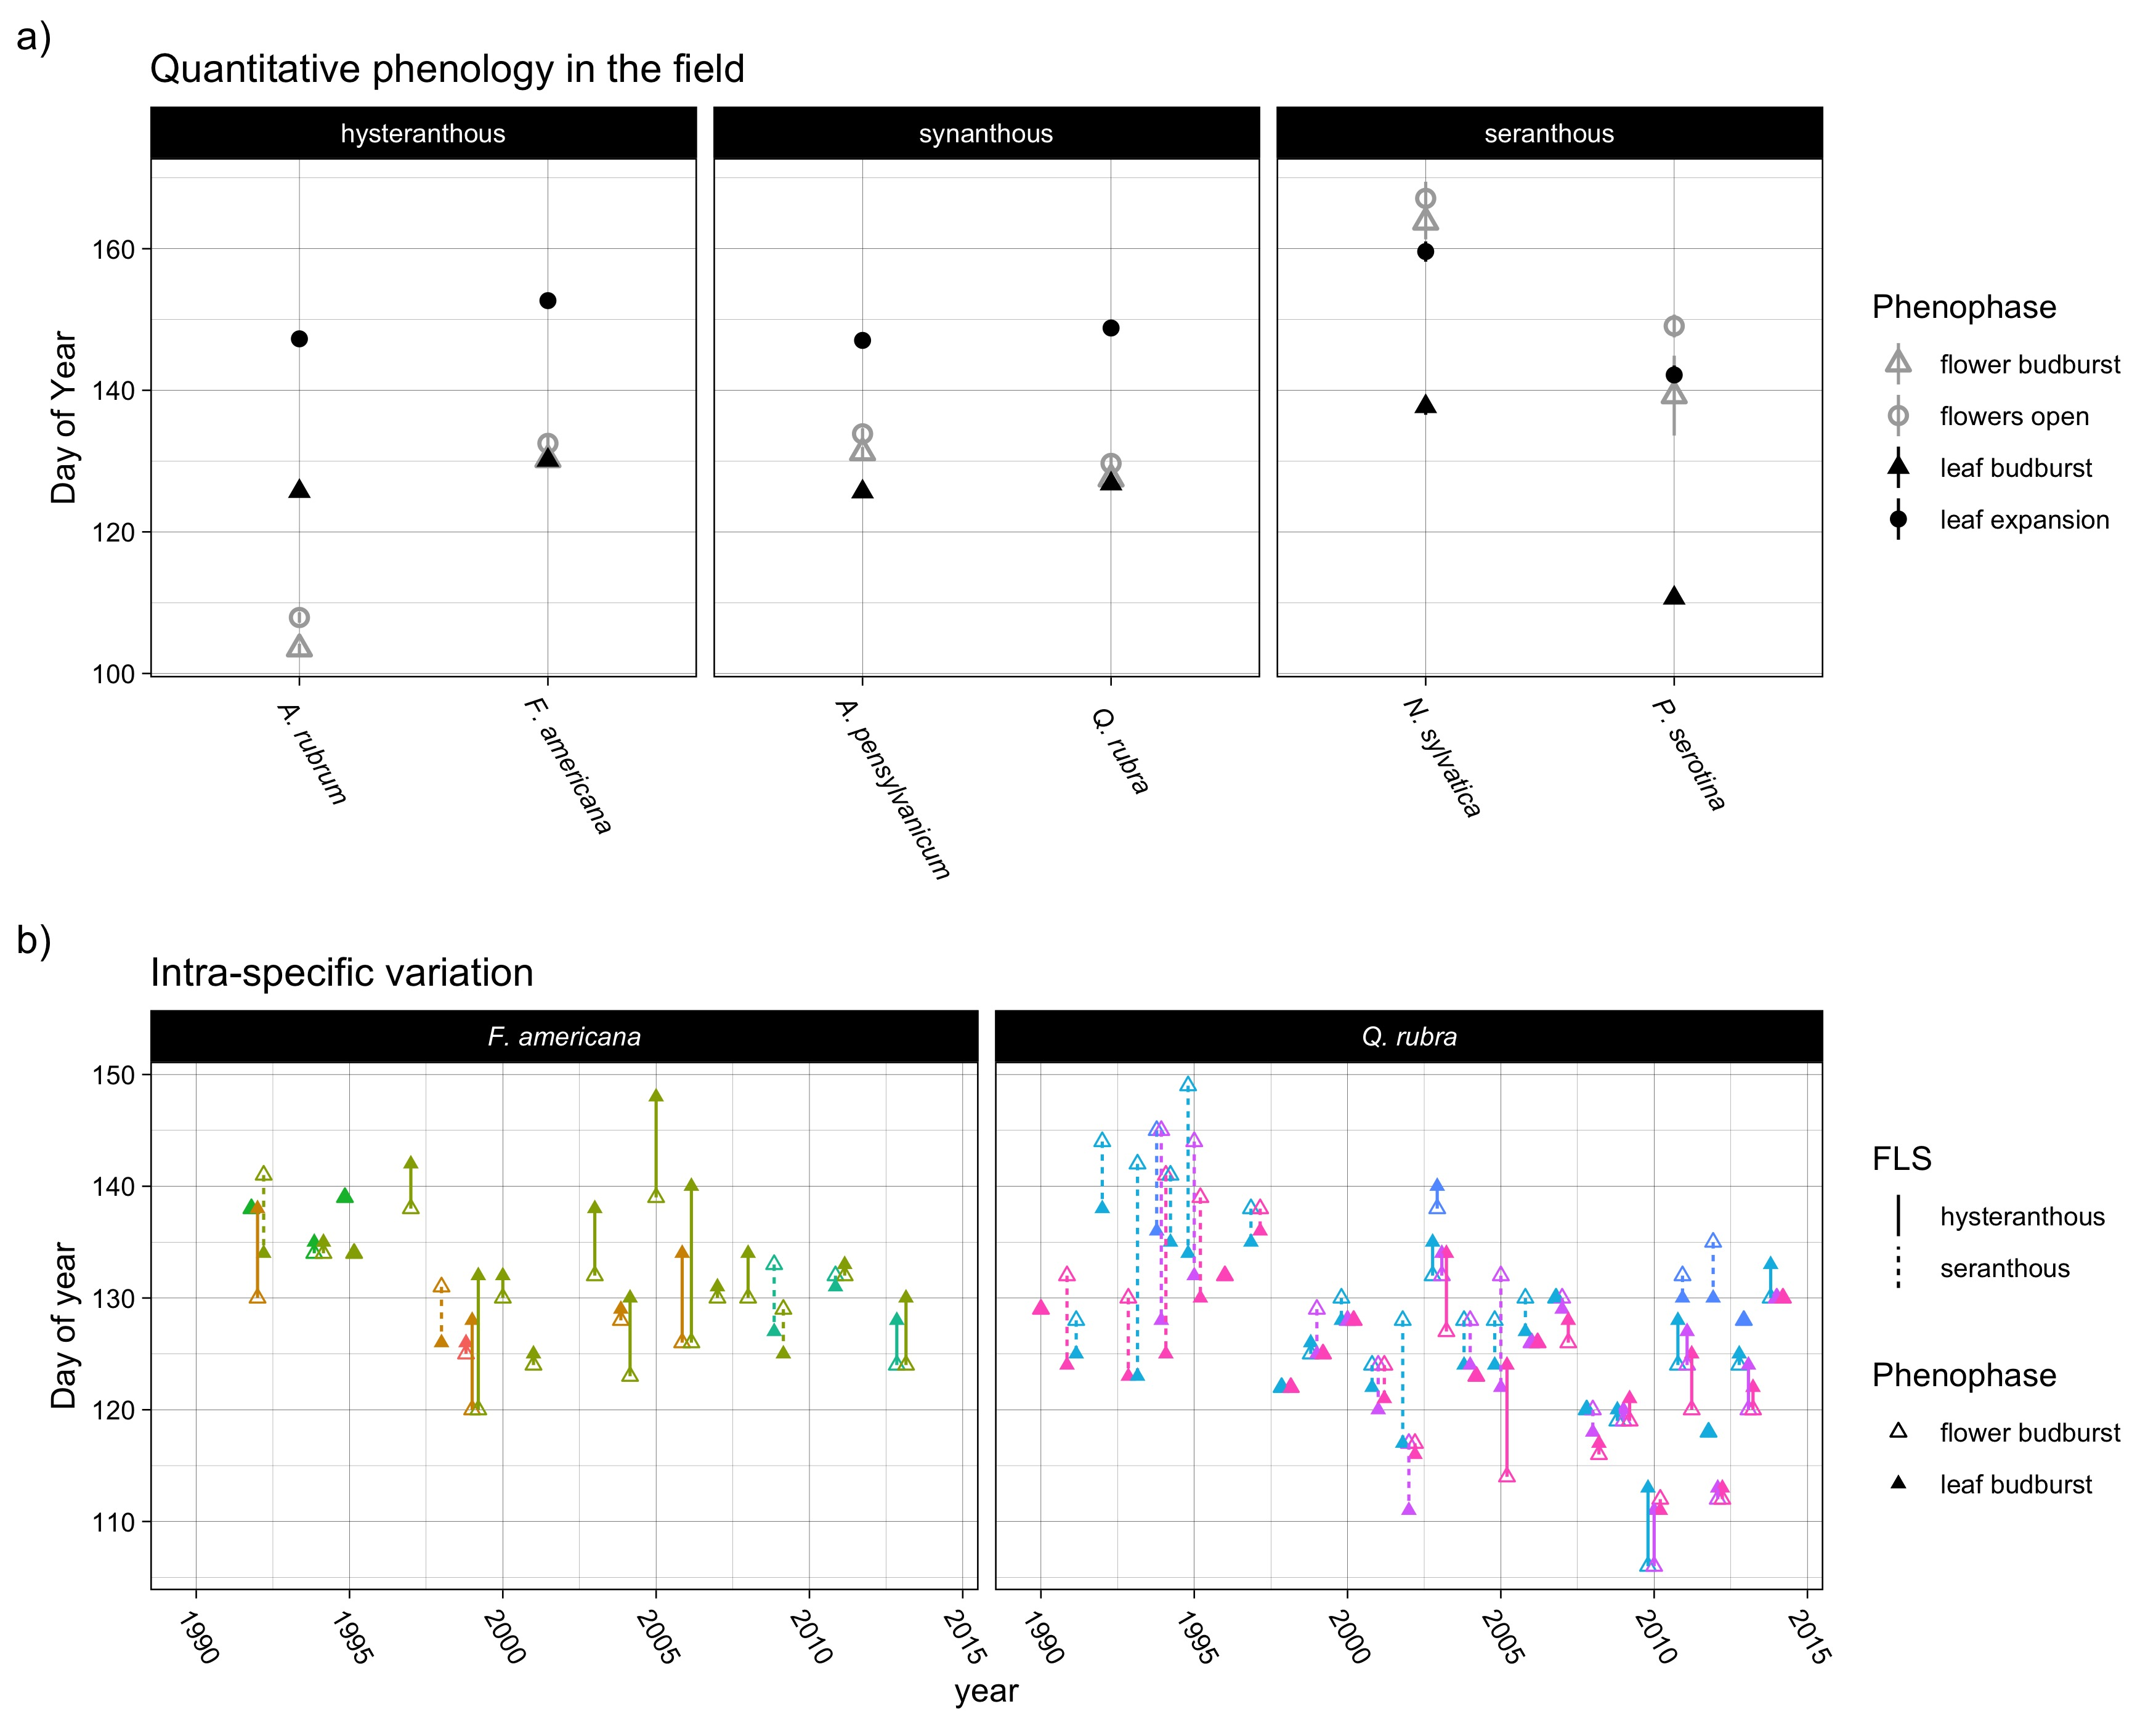
\includegraphics[width=\textwidth]{..//HarvardForest/FLS_viz.jpeg}
          \caption{\textbf{The shift from catagorical/interspecific descriptions to qunatitative/intra-specific measures of FLS reveals substantial, previously unrecognized variation.} Under the current framework, species are assigned to FLS categories by the order of phenophases alone (Fig. a.). However,  measuring the time between phenophases reveals substantial differences amoung species within each category (Fig. b.), obscured by categorization. Below the species level, the time between flowering and leaf activity also can vary by as much as several weeks between individuals and years, with, for some species, the sequence itself regularly switching across time and between individuals (Fig. c.). This inter- and intra- specific variation is key understandimg the function of FLS variation in deciduous, woody plants}
        \label{fig:vizzy}
    \end{figure}
    
 \begin{figure}[h!]
        \centering
          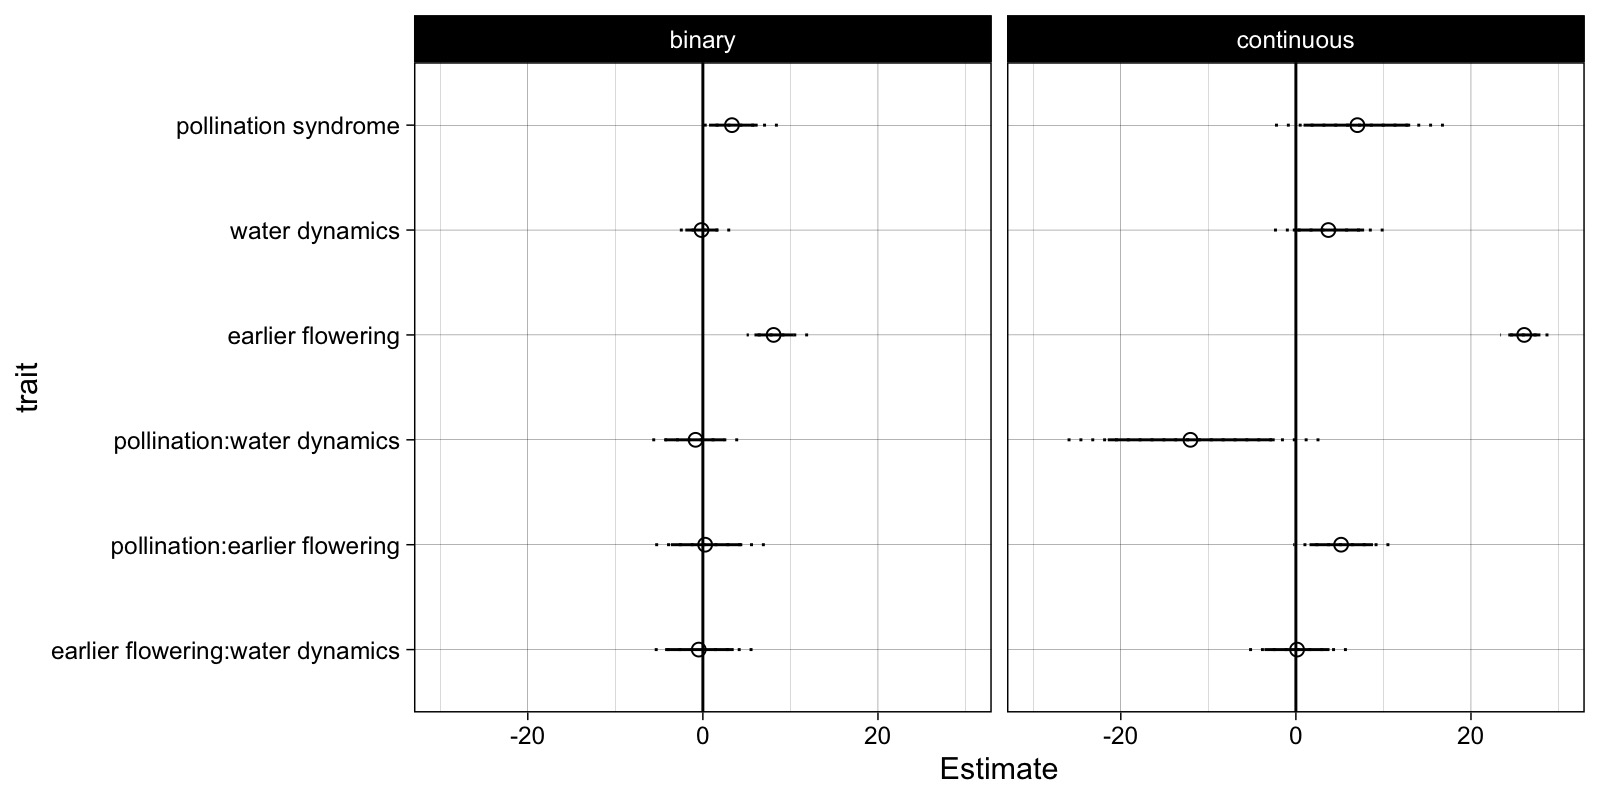
\includegraphics[width=\textwidth]{..//HF.jpeg}
          \caption{\textbf{Mean estimates of the effects of FLS predictors on the timing between flowering and leaf expansion for indivual woody plants at Harvard Forest between 1990-2015 reveal important differences between catagorical and quantitative frameworks of FLS.}  With the catagorical approach, there is a strong effect of flowering time and pollination syndrome on FLS variability, with no detectable effect of water dynamics or interactions between the predictors. However, with quantitatve measures of FLS, we find increased support for the water dynamics hypothesis, and strong interactions between pollination syndrome and both flowering time and water dynamics. This interactions suggest multiple drivers of FLS varaibility in the temperate zone.  Both models use a Bayesian, phylogenetic mixed modeling approach with standardized predictors to allow for comparisions between then.  Lines represent 50 and 95\% credible intervals.}  
        \label{fig:muplots.HF}
    \end{figure}    

    

 \begin{figure}[h!]
        \centering
          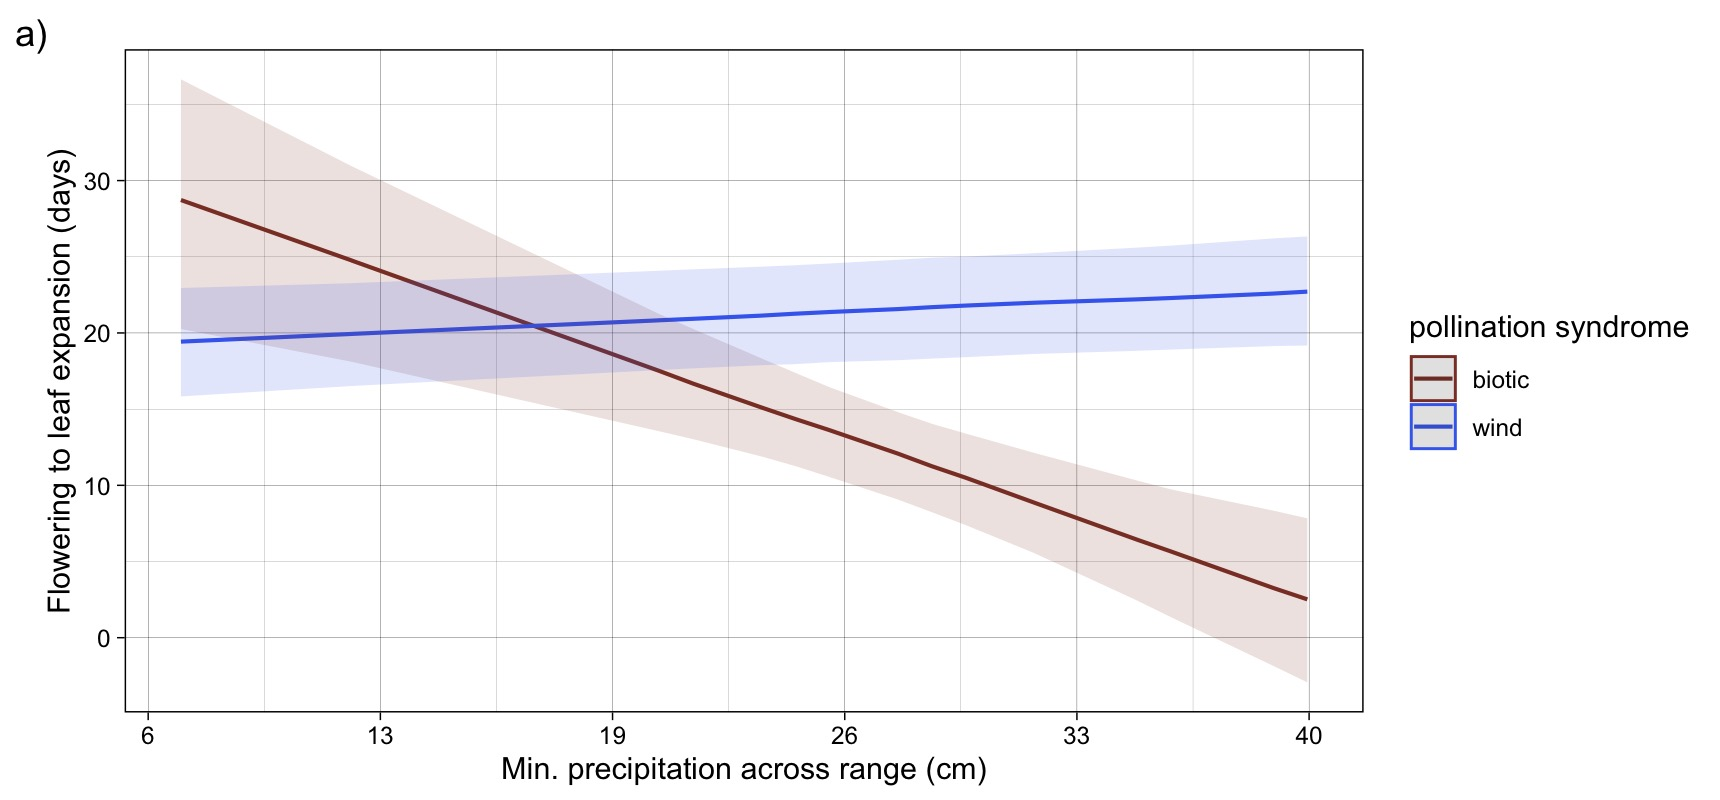
\includegraphics[width=\textwidth]{..//HarvardForest/apcs.jpeg}
           \caption{\textbf{ For indiviudals flowering in early May, marginal effects from our qunatitative FLS model suggest that water dynamics may be a driver of hysteranthy in biotically-pollinated but not in wind-pollinated taxa.}  These systematic differences in drivers of FLS reflect greater differences in the bio-geographic histories of the wind and biotcally-pollinated taxa of temperate forest communities.}
        \label{fig:apcs}
    \end{figure}
 

    
\end{document}
